\documentclass[oneside]{article}

\usepackage{wallpaper}
\usepackage{geometry}
\usepackage[
    unicode=true,
    bookmarks=true,
    bookmarksnumbered=false,
    bookmarksopen=true,
    bookmarksopenlevel=1,
    breaklinks=false,
    pdfborder={0 0 0},
    backref=false,
    colorlinks=false
]{hyperref}
\usepackage{lastpage}
\usepackage{hyphenat}
\usepackage{hyphsubst}
\usepackage{tabularx}
\usepackage{moresize}
\usepackage[document]{ragged2e}

\usepackage[scaled]{helvet}
\usepackage{fontawesome5} 
\usepackage{tikz}
\usepackage[defaultfam,tabular,oldstyle]{montserrat}
\usepackage[T1]{fontenc}
\renewcommand*\oldstylenums[1]{{\fontfamily{Montserrat-TOsF}\selectfont #1}}

\usepackage{titlesec}
\usepackage{xcolor}

\setlength{\parindent}{0pt}
\titleformat{\section}{\normalfont}{}{0pt}{}

\renewcommand{\arraystretch}{1.2}

\setlength\fboxrule{0pt}
\setlength\fboxsep{8pt}

\titlespacing{\section}{0pt}{1ex plus .1ex minus .2ex}{1ex}

\newcolumntype{Y}{>{\RaggedRight\arraybackslash}X}

\hypersetup{
    pdftitle={Rémy Jovanovic - CV - French},
    pdfauthor={Rémy Jovanovic},
    pdfsubject={CV}
}

\geometry{
    a4paper,
    left=10pt,
    right=10pt,
    top=10pt,
    bottom=10pt,
    nohead,
    nomarginpar
}

\definecolor{sidebg}{cmyk}{0.57, 0.91, 0, 0.34}
\definecolor{mainbg}{cmyk}{0, 0, 0, 0}

\usepackage{eso-pic}
\AddToShipoutPictureBG{%
    \AtPageLowerLeft{%
        \color{sidebg}\rule{\paperwidth}{\paperheight}%
    }%
}
\definecolor{maintext}{cmyk}{1, 0.02, 0, 0.8}
\definecolor{sidetext}{cmyk}{0, 0, 0.07, 0.04}

\pagecolor{mainbg}

\begin{document}
\setlength{\topskip}{0pt}\setlength{\footskip}{0pt}%
\fcolorbox{red}{sidebg}{%
    \begin{minipage}[t][\textheight-2\fboxsep-2\fboxrule][t]{\dimexpr0.40\textwidth-2\fboxrule-2\fboxsep\relax}
        \color{sidetext}
        {\bfseries\scshape\HUGE JOVANOVIC} \\
        {\bfseries\scshape\Huge Rémy}
        \begin{center}
            \begin{tikzpicture}
                \clip (0,0) circle (1.9cm);
                \node[anchor=center] at (0,0) {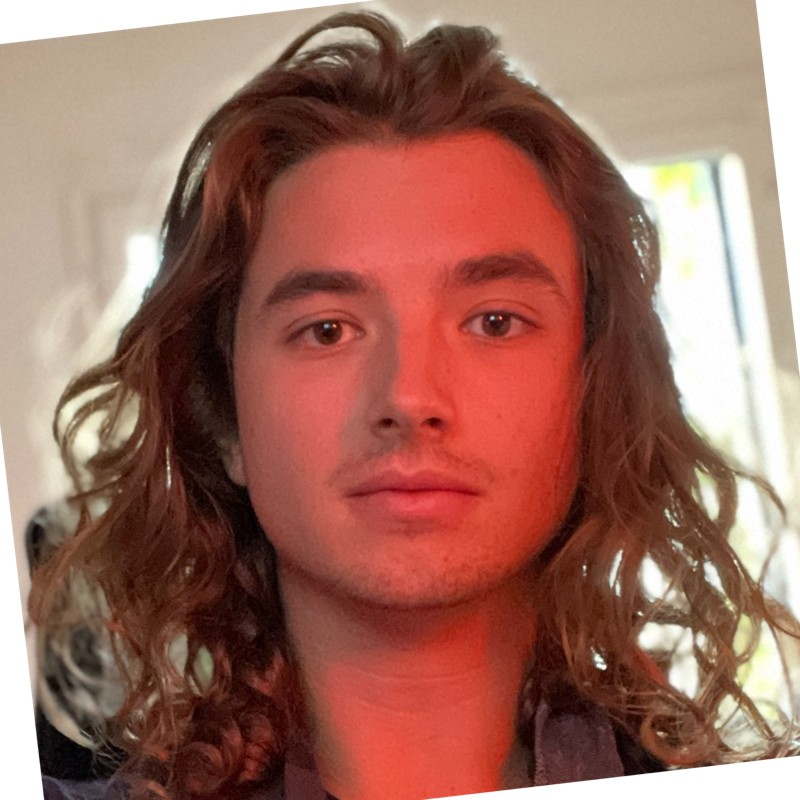
\includegraphics[width=4cm]{images/profile.jpg}};
                \draw[thick, color=black] (0,0) circle (1.9cm);
            \end{tikzpicture}
        \end{center}
        \vspace{.2cm} \\
        Étudiant en Ingénierie Système d'Information
        \vspace{.2cm}
        \phantomsection{}
        \addcontentsline{toc}{section}{Mes Informations}
        \section*{\large Mes Informations \\
        \rule{\linewidth}{0.4pt}}
        \begin{tabularx}{\textwidth}{cY}
            \faMapMarker{}  & 1 impasse du pavillon, 78930 \\
            & Villette \\
            \faPhone{}      & 06 52 22 44 39 \\
            \faEnvelope{}   & \href{mailto:remyj@outlook.fr}{remyj@outlook.fr} \\
            \faGithub{}   & \href{https://github.com/aym00n-djrak}{aym00n-djrak} \\
            \faLinkedin{}   & Rémy JOVANOVIC \\
            \faUser{}       & Root-me: Score 195pts \\
            \faCar{}        & Permis B \\
        \end{tabularx}
        \vspace{.3cm} \\
        \phantomsection{}
        \addcontentsline{toc}{section}{Compétences}
        \section*{\scshape\Large Compétences \rule{\ linewidth}{0.4pt}}
        \begin{tabularx}{\textwidth}{cY}
            \faCode{}        & C, C\#, Java, Python, JS, TS, PHP \\
            \faLaptopCode{}  & Git, Docker, GitLab CI/CD \\
            \faDatabase{}    & SQL, PostgreSQL, NoSQL \\
            \faCodeBranch{}  & Java: Spring, Hibernate, Spring Boot \\
            \faDesktop{}     & Front-end: JavaScript, React, Angular \\
            \faLink{}        & Blockchain : Décentralisation, Wallet, Pool, Transactions, Cryptographie \\
            \faBrain{}       & Machine Learning: Régression Linéaire, FFNN, K-Means \\
            \faNetworkWired{} & Cisco Packet Tracer, Wireshark \\
            \faLinux{}       & Gentoo, Debian \\
        \end{tabularx}
        \vspace{1pt} \\
        \phantomsection{}
        \phantomsection{}
        \addcontentsline{toc}{section}{langues}
        \section*{\scshape\Large Langues  \\
        \rule{\linewidth}{0.4pt}}
        \begin{tabular}{cl}
            \faLanguage{} & Français (langue maternelle) \\
            \faLanguage{} & Anglais (niveau B2) \\
            \faLanguage{} & Mandarin (niveau A2)
        \end{tabular}
        \vspace{.3cm}
        \\        
        \phantomsection{}
        \addcontentsline{toc}{section}{Certifications}
        \section*{\scshape\Large Certifications \rule{\linewidth}{0.4pt}}
        \begin{tabular}{cl}
            \faCertificate{} & Takima - Certification Java Master 3 \\
            \faCertificate{} & TOEIC - 925 \\
            \faCertificate{} & MOOC - Gestions de Projet
        \end{tabular}
        \vspace{.3cm}
    \end{minipage}
}
\fcolorbox{red}{mainbg}{%
    \begin{minipage}[t][\dimexpr\textheight-2\fboxrule-2\fboxsep\relax][t]{\dimexpr0.6\textwidth-2\fboxrule-2\fboxsep\relax}
        \color{maintext}
        \phantomsection{}
        \addcontentsline{toc}{section}{Expériences Professionnelles}
        \section*{\scshape\Large Expériences Professionnelles \rule{\linewidth}{0.4pt}}
%
        {\large \textbf{Takima}} \\ 
        {{\fontseries{medium}\selectfont Stage Ingénieur Développeur Fullstack}} \\
        {\scshape\fontseries{light}\selectfont\footnotesize Mars 2024 \textendash{} Août 2024} 
        \begin{itemize}
            \setlength{\itemsep}{-2pt}
            \item Participation aux cérémonies Agile: Scrum, Sprint Planning, Sprint Review, Sprint Retrospective, Daily Scrum
            \item Intégration dans une équipe fullstack, implémentation de nouvelles fonctionnalités (projet App-User)
            \item Technologies utilisées: Git, Java, Maven, Spring, Hibernate, Spring Boot, Javascript, Docker
            \item Certification Java
        \end{itemize}
%
        {\large \textbf{CS GROUP}} \\
        {{\fontseries{medium}\selectfont Stage Ingénieur, Intégration et Validation Système}} \\
        {\scshape\fontseries{light}\selectfont\footnotesize Avril 2023 \textendash{} Août 2023} 
        \begin{itemize}
            \setlength{\itemsep}{-2pt}
            \item Mise en place d'une plateforme utilisant la VoIP
            \item Intégration et validation d'un système radio VoIP
        \end{itemize}

        \phantomsection{}
        \addcontentsline{toc}{section}{Formation Scolaire}
        \section*{\scshape\Large Formation Scolaire \\
         \rule{\linewidth}{0.4pt}}
%
        {\large \textbf{Rotterdam University of Applied Sciences}} \\ 
        {{\fontseries{medium}\selectfont Erasmus, module Blockchain}} \\
        {\scshape\fontseries{light}\selectfont\footnotesize 2023/2024} 
        \\[1ex]

        {\large \textbf{École Centrale d'Électronique de Paris}} \\ 
        {{\fontseries{medium}\selectfont Diplôme d'Ingénieur, majeure Système d'Information}} \\
        {\scshape\fontseries{light}\selectfont\footnotesize 2021/2024} 
        \\[1ex]

        {\large \textbf{CPGE}} \\ 
        {{\fontseries{medium}\selectfont Classe préparatoire scientifique, MP, option informatique}} \\
        {\scshape\fontseries{light}\selectfont\footnotesize 2020/2021} 
        \\[1ex]

        \phantomsection{}
        \addcontentsline{toc}{section}{Projets Scolaire}
        \section*{\scshape\Large Projets Scolaire\\
         \rule{\linewidth}{0.4pt}}
        \begin{justify}
        \setlength{\parindent}{0pt}

        {\large \textbf{Prototype de Blockchain}} \\
        {\scshape\fontseries{light}\selectfont\footnotesize Python, Socket programming, P2P} \\
        Implémentation d'une blockchain en Python
        Réalisation d'un wallet, ou l'on peut envoyer et recevoir des transactions, miner des blocs, et consulter la blockchain entre pairs.
        \\[1ex]

        {\large \textbf{Cardiofréquencemètre}} \\
        {\scshape\fontseries{light}\selectfont\footnotesize Arduino, C++} \\
        Mesure de la tension, affichage et stockage dans la mémoire EEPROM
        \\[1ex]

        {\large \textbf{Reconnaissance vocale}} \\
        {\scshape\fontseries{light}\selectfont\footnotesize Arduino, C++} \\
        Apprentissage et reconnaissance vocale des mots 1-2 et 3 à partir d’une Arduino nano
        \\[1ex]

        {\large \textbf{Omnes Santé}} \\
        {\scshape\fontseries{light}\selectfont\footnotesize JS, PHP, HTML, CSS} \\
        Site web de mise en relation client/docteur, prise de rendez-vous, visioconférence et messagerie intégrée
        \\[1ex]

        {\large \textbf{Portfolio}} \\
        {\scshape\fontseries{light}\selectfont\footnotesize React, JavaScript, Supabase, NextJS} \\
        Portfolio Single Page Application, avec un formulaire de contact, un blog, et une gestion d'articles
        \\[1ex]
        \end{justify}
    \end{minipage}
}
\end{document}
